% A (little more than a) minimal working example
\documentclass[12pt, a4paper]{article}

% Increase tex widht and heigh by 4cm
\addtolength{\textwidth}{4cm}
\addtolength{\oddsidemargin}{-2cm}
\addtolength{\textheight}{4cm}
\addtolength{\topmargin}{-2cm}

% To start out let's include the following packages
\usepackage[utf8]{inputenc} % encoding
\usepackage{hyperref} % for clickable references
\usepackage{xcolor} % custom colors
\usepackage{graphicx} % for including graphics
\usepackage{pgfplots} % for plots and more
\usepackage{tikz} % for drawing and more
\usepackage{booktabs} % for nice tables
\usepackage{amsmath} % math stuff
\usepackage{amsfonts}
\usepackage{amssymb}
\usepackage{float}
\usepackage{listings}

\begin{document}

\title{%
	{\bfseries All about Processors}\\[1ex] % your title goes here
	{\large\bfseries A closer look on what is inside a processing unit and how it works} % if you want to use a subtitle...
}
\author{Philip Lukert} % your name

\date{\vspace{-5ex}} % dirty hack to remove date from titlepage

{\sf \maketitle} % use serif free font for title page

\begin{center}
	
\includegraphics[width=8cm]{logo_sdv.pdf}\\
	{\large\sf Sommerakademie in Leysin, August 2016}
\end{center}

\vspace{1cm}

\begin{abstract}
Für meine Präsentation in der Gruppe "Energieeffizientes Rechnen" habe ich mich mit dem Aufbau eines Prozessors auseinandergesetzt. Diese Erkenntnisse werde ich im folgenden Paper kurz zusammenfassen. Als erstes werde ich auf grundlegende logische Schaltungen eingehen und wie man daraus einen Baustein baut, der zwei Zahlen addiert. Bevor ich zum eigentlichen Prozessor komme, muss ich noch eine kurze Einführung in die Assemblersprache MIPS einschieben, um im Anschluss den Aufbau eines MIPS-Prozessors illustrieren zu können. Am Ende werde ich noch auf Verbesserungen, wie beispielsweise Pipelining eingehen.
\end{abstract}

% The table of contents
\newpage
\tableofcontents
\newpage



\section{Addierer}
In diesem Abschnitt werde ich erläutern, was Transistoren sind und wie man daraus einen Schaltkreis baut, der zwei Zahlen addieren kann.


\subsection{Transistoren}
\begin{figure}[H]
	\begin{center}
		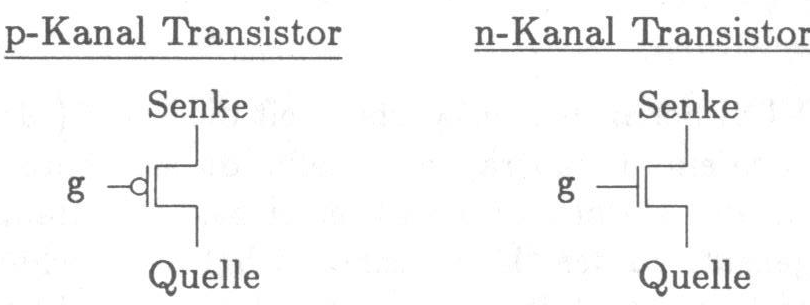
\includegraphics [width=14cm]{Transistoren.png}
	\end{center}
	\caption{p- und n-Kanal Transistoren}
\end{figure}
Transistoren kann man sich als elektronische Schalter vorstellen. Sie haben eine Quelle, eine Senke und ein Gate. Das Gate bestimmt, ob Strom von der Quelle zur Senke fließen kann. Der n-Kanal Transistor rechts leitet den Strom, falls eine ausreichend hohe Spannung anliegt. Bei dem linken p-Kanal Transistor ist es genau anders herum, er leitet, falls keine Spannung anliegt. Informatiker abstrahieren "Spannung" zu 1 und "keine Spannung" zu 0. Zwischenstände sind also eher unerwünscht und werde ich in diesem Paper nicht behandeln.


\subsection{Logische Gatter}
Logische Gatter sind Schaltungen, die für bestimmte Eingaben bestimmte Ausgaben produzieren. Für jede Schaltung kann man eine Wahrheitstabelle aufstellen. Diese sieht z.B. für ein NOT-Gatter folgendermaßen aus:

\begin{table}[H]
	\begin{center}
		\begin{tabular}{|c|c|} \hline
			Eingabe & Ausgabe \\ \hline
			1 & 0 \\
			0 & 1 \\ \hline
		\end{tabular}\\
	\end{center}
	\caption{NOT Wahrheitstabelle}
\end{table}

Dieses logische Gatter kann man aus zwei Transistoren zusammenbauen:

\begin{figure}[H]
	\begin{center}
		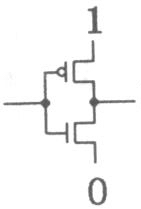
\includegraphics [width=4cm]{NOT.png}
	\end{center}
	\caption{NOT-Gatter}
\end{figure}

Links ist der Eingang und rechts der Ausgang. Oben und unten liegen eine 1 und eine 0 an (also beispielsweise 5V und 0V). Falls am Eingang ein Signal anliegt, verbindet der untere n-Kanal Transistor die 0 mit dem Ausgang. Der obere p-Kanal Transistor blockiert dagegen. Das bedeutet, dass zu der Eingabe 1 die Ausgabe 0 folgt, wie in der ersten Zeile der Wahrheitstabelle beschrieben. Falls eine 0 anliegt, ist es genau anders herum. Der untere Transistor sperrt, während der obere Transistor die 1 mit dem Ausgang verbindet.

Ähnlich, wie dieses NOT-Gatter kann man alle üblichen logischen Schaltungen aus Transistoren konstruieren. 

\begin{figure}[H]
	\begin{center}
		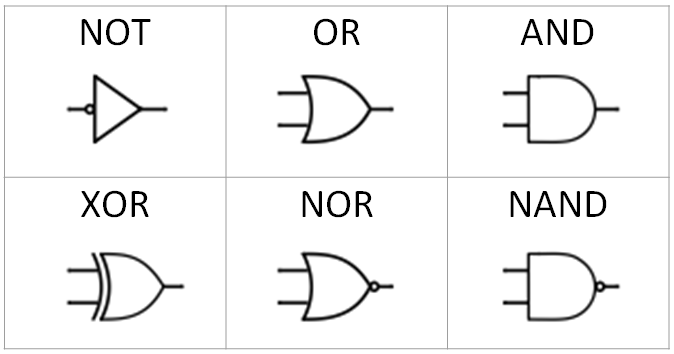
\includegraphics [width=10cm]{Gatter.png}
	\end{center}
	\caption{die wichtigsten grundlegenden Gatter}
\end{figure}

Ab jetzt werde ich nur noch mit diesen Gattern arbeiten und keine Transistoren mehr erwähnen.


\subsection{Addierer}
In diesem Abschnitt werde ich zeigen, wie man mit diesen Gattern einen Addierer baut, also einen Schaltkreis, der zwei Zahlen addiert.
Da die Gatter nur binäre Ein- und Ausgänge besitzen, d.h. sie haben entweder 0 oder 1 als Ein/Ausgang, muss man die Zahlen binär kodieren. Hier gehe ich davon aus, dass dies dem Leser schon bekannt ist. Als kleines Beispiel: 1001 binär kodiert entspricht 8*\textbf{1} + 4*\textbf{0} + 2*\textbf{0} + 1*\textbf{1} = 9

Mit dieser binären Kodierung kann man also folgende Grobskizze von dem gewünschten Addierer anfertigen:

\begin{figure}[H]
	\begin{center}
		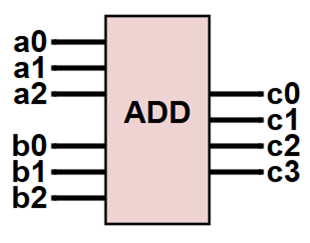
\includegraphics [width=6cm]{Addierer.png}
	\end{center}
	\caption{Ein Schaltkreis, der addieren soll: \ Links werden zwei Zahlen mit je 3 Bit einglesen, worauf rechts eine Zahl mit 4 Bit ausgegeben wird. Das Ergebnis hat 4 Bit, da, wenn man 2 3-Bit Zahlen addiert, eine 4-Bit Zahl als Ergebnis herauskommen kann. Dieses Phänomen des Überlaufs werde ich später noch ausfürlicher erläutern.}
\end{figure}


\subsection{Halbaddierer}
Als ersten Schritt baut man einen Addierer, der zwei Zahlen mit je einem Bit zu einer Zahl mit zwei Bit addiert. Dies nennt man Halbaddierer. Dazu kann man folgende Wahrheitstabelle aufstellen:

\begin{table}[H]
	\begin{center}
		\begin{tabular}{|c|c|c|c|} \hline
			A & B & C & dezimal \\ \hline
			0 & 0 & 00 & 0+0=0 \\
			0 & 1 & 01 & 0+1=1 \\
			1 & 0 & 01 & 1+0=1 \\
			1 & 1 & 10 & 1+1=2 \\ \hline
		\end{tabular}\\
	\end{center}
	\caption{Halbaddierer Wahrheitstabelle}
\end{table}

Mit dieser Wahrheitstabelle kann man folgende Schaltung konstruieren:

\begin{figure}[H]
	\begin{center}
		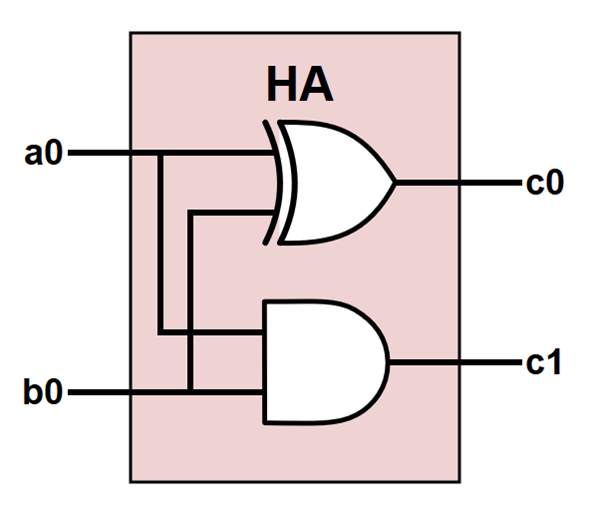
\includegraphics [width=7cm]{Halbaddierer.png}
	\end{center}
	\caption{Ein Halbaddierer}
\end{figure}

Wie bereits zuvor erwähnt, hat das Ergebnis ein Bit mehr, als die Eingaben. Dieses eine Bit nennt man Übertrag. Wenn man jetzt mehrere Halbaddierer verwenden will, um einen Addierer mit mehr als einem Bit konstruieren will, stellt man fest, dass man diesen Übertrag wie bei der schriftlichen Addition aus der Grundschule in die nächste "Rechnung", also in den nächsten Halbaddierer mit einbeziehen muss. Dies nennt sich nicht mehr Halbaddierer, sondern Volladdierer.

\subsection{Volladdierer}
Bei dem Volladdierer werden nicht nur zwei mal ein Bit addiert, sondern drei mal ein Bit. Das dritte Bit ist der Übertrag aus dem vorherigen Halb/Volladdierer. Dafür sei unten die Wahrheitstabelle angegeben. 

\begin{table}[H]
	\begin{center}
		\begin{tabular}{|c|c|c|c|c|} \hline
			a&b&c&out&dezimal \\ \hline
			0&0&0&00&0+0+0=0 \\
			0&0&1&01&0+0+1=1 \\
			0&1&0&01&0+1+0=1 \\
			0&1&1&10&0+1+1=2 \\
			1&0&0&01&1+0+0=1 \\
			1&0&1&10&1+0+1=2 \\
			1&1&0&10&1+1+0=2 \\
			1&1&1&11&1+1+1=3 \\ \hline
		\end{tabular}\\
	\end{center}
	\caption{Volladdierer Wahrheitstabelle}
\end{table}

Wie beim Halbaddierer kann man auch für einen Volladdierer eine logische Schaltung konstruieren. Die HA-Blöcke sind hierbei Halbaddierer.

\begin{figure}[H]
	\begin{center}
		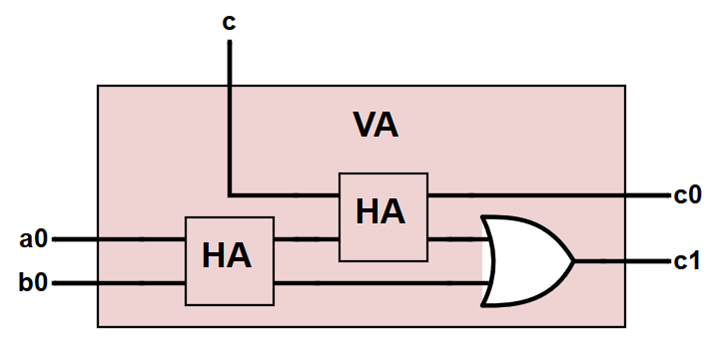
\includegraphics [width=10cm]{Volladdierer.png}
	\end{center}
	\caption{Ein Volladdierer}
\end{figure}

Jetzt kann man aus mehreren Volladdierern einen kompletten n-Bit Addierer bauen. Dabei wird der Übertrag vom vorherigen Volladdierer wie in der Abbildung an den nächsten Volladdierer übergeben.

\begin{figure}[H]
	\begin{center}
		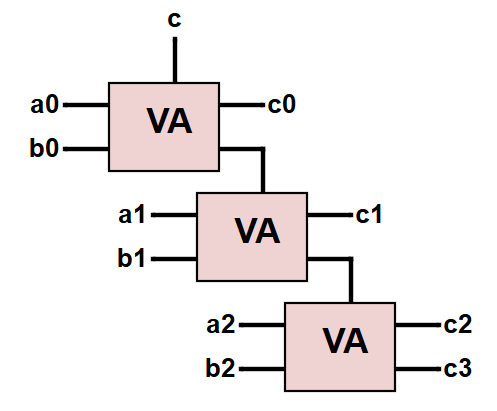
\includegraphics [width=10cm]{VolladdiererHintereinander.png}
	\end{center}
	\caption{3 Volladdierer zu einem 3-Bit Addierer verschaltet; Der Übertrag, den der erste Volladdierer bekommt, wird in diesem Fall nicht gebraucht. Jedoch kann er für die Subtraktion von Zahlen sehr nützlich sein.}
\end{figure}


\section{MIPS}
In diesem Abschnitt werde ich eine kurze Einführung in MIPS geben, damit ich den Aufbau des Prozessors danach besser erklären kann. Mips ist eine Assembler-Programmiersprache, die recht einfach aufgebaut ist. Hier ein kleines Beispielprogramm:

\begin{figure}[H]
	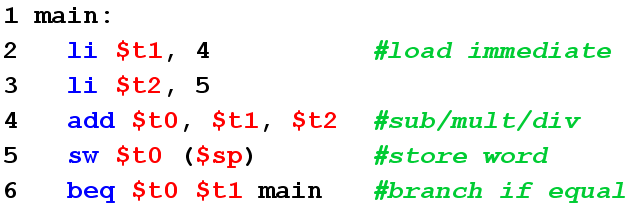
\includegraphics [width=10cm]{MIPS.png}
\end{figure}

Das Wichtigste bei MIPS sind die 32 Register. Das sind kleine Speicherzellen, auf die sehr schnell zugegriffen werden kann. Jedes Register hat einen Namen, z.B. \textbf{t0}, \textbf{t1}, \textbf{t2} oder \textbf{sp}. Ein Register kann im Code mit \textbf{\$Name} angesprochen werden. Der Befehl in Zeile 2 ist z.B. ein load-immediate Befehl. Mit ihm kann ein Zahlenwert in ein Register geladen werden. In diesem Fall wird die 4 in das Register \textbf{t1} geladen. In Zeile 4 wird eine Rechenoperation ausgeführt. Hier werden die Zahlen, die in den Registern \textbf{t1} und \textbf{t2} stehen, addiert und in \textbf{t0} abgespeichert. Damit ist die Sprache schon sehr mächtig. Jedoch bieten 32 Register nur beschränkte Möglichkeiten. Dafür gibt es den Arbeitsspeicher, in den bei MIPS bis zu 4GB Speicher passen. Um mit ihm zu kommunizieren, gibt es den Befehl sw für store-word. In Zeile 5 wird der Inhalt von \textbf{t2} an die Adresse \textbf{sp} (\textbf{sp} ist ein Register) gespeichert. Das heißt, dass jetzt eine 9 an der Stelle \textbf{sp} im Arbeitsspeicher stehen müsste. Die letzte Struktur, die ich hier erklären werde, sind Sprünge. Wie vielleicht schon aufgefallen ist, ist in der ersten Zeile eine Marke namens "main". In Zeile 6 ist die bedingte Sprungoperation branch-if-equal. Sie wird "angewendet", wenn der Wert von \textbf{t0} gleich \textbf{t1} ist. In diesem Fall wird also nicht zu der Marke main in Zeile 1 gesprungen.


\section{Prozessor}
In diesem Abschnitt wende ich mich wieder der Hardware zu. Ich werde erläutern, wie man von dem Addierer, den ich bereits detailliert erklärt habe, zu einem funktionierenden Computer kommt.

\begin{figure}[H]
	\begin{center}
		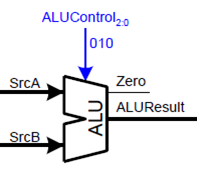
\includegraphics [width=4cm]{ALU.png}
		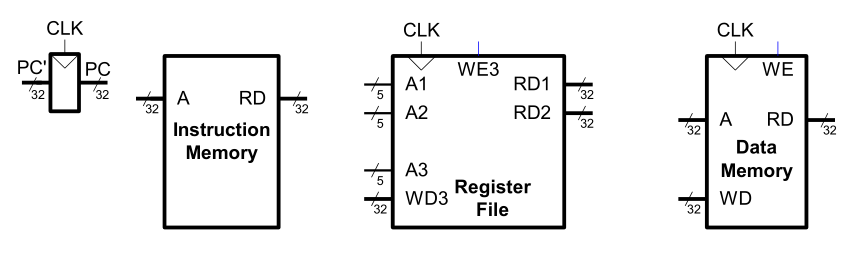
\includegraphics [width=13cm]{Prozessor0.png}
	\end{center}
	\caption{Bauteile eines MIPS-Prozessors}
\end{figure}

Das wichtigste an einem Prozessor ist die ALU (Arithmetic Logic Unit) links. In ihr steckt u.a. der Addierer. Jedoch kann die ALU noch mehr Rechenoperationen, als nur addieren. Mit der ALU-Control Leitung wird angegeben, welche Rechenoperation die ALU momentan ausführen soll. Den zusätzlichen Zero-Ausgang werde ich später noch einmal ansprechen.

Rechts neben der ALU ist der ProgramCounter (PC). Dies ist eine kleine Speicherzelle, die speichert, welche Zeile Code (MIPS) das Programm als nächstes ausführen soll. Normalerweise wird er immer um eine Zeile erhöht, wenn ein Befehl abgearbeitet wurde. Nur bei Sprunginstruktionen, wie in der letzten Zeile den Beispielprogramms in Mips, wird er anderweitig verändert.

Ich habe den Instruktions-Speicher und den Daten-Speicher hier der Einfachheit halber getrennt. Sie verfügen über Eingänge, um die Adresse anzugeben, an der der Speicherinhalt gelesen werden soll und über einen Ausgang, an dem im Anschluss die Daten von der eingegebenen Adresse anliegen. Der Datenspeicher hat zusätzlich noch einen Write-Eingang, mit dem Daten in den Speicher geschrieben werden können.

Als letztes fehlen noch die 32 Register. Dieser Block hat mehr Ein- und Ausgänge, damit gleichzeitig 2 Daten gelesen werden können und ein Datum geschrieben werden kann. z.B. beim ADD Befehl werden aus zwei Registern Daten gelesen, diese werden addiert und dann in das dritte Register geschrieben.\\

Im Folgenden werde ich anhand von diesen Bausteinen durch die einzelnen Phasen einer Instruktionsausführung gehen um diese einzeln zu erklären.

\subsection{Instruction-Fetch Phase}
\begin{figure}[H]
	\begin{center}
		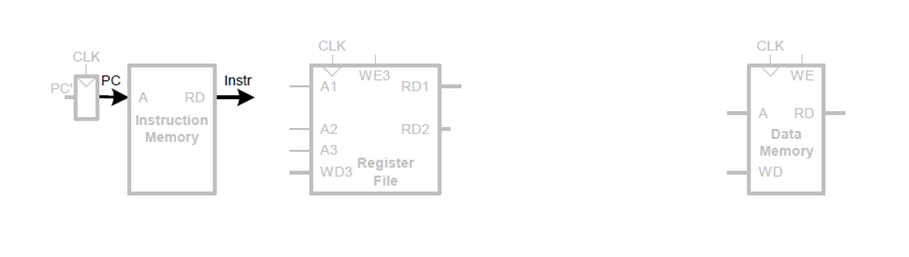
\includegraphics [width=17cm]{Prozessor1.png}
	\end{center}
	\caption{Instruction-Fetch}
\end{figure}

Beim Instruction-Fetch wird aus dem PC die Adresse geholt, an der der nächste Befehl gespeichert ist. Mit dieser Adresse wird dann auf den Befehls-Speicher zugegriffen und der aktuelle Befehl wird geladen.

\subsection{Register-Fetch Phase}
\begin{figure}[H]
	\begin{center}
		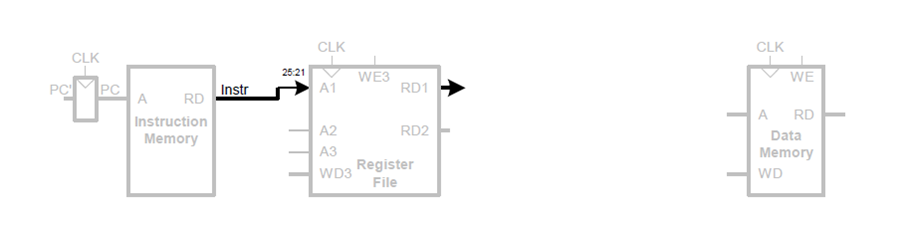
\includegraphics [width=17cm]{Prozessor2.png}
	\end{center}
	\caption{Register-Fetch}
\end{figure}

Der Befehl, der aus dem Befehls-Speicher geladen wurde, ist in 32Bit kodiert. Die Bits 25 bis 21 beispielsweise speichern die Adresse des Registers, aus dem die Daten geladen werden sollen. Diese werden in der Register-Fetch Phase geladen und liegen im folgenden am Ausgang des Register Bausteins an.

\subsection{Execute Phase}
\begin{figure}[H]
	\begin{center}
		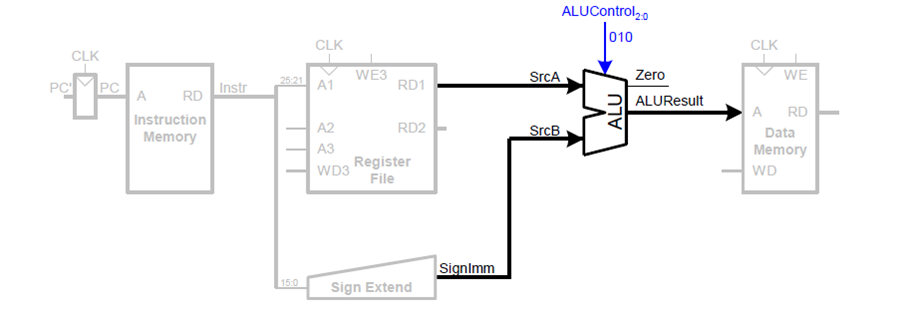
\includegraphics [width=17cm]{Prozessor3.png}
	\end{center}
	\caption{Execute}
\end{figure}

In der Execute-Phase werden zwei Datenströme in die ALU geschickt, die dann eine bestimmte Rechenoperation ausführen soll. In diesem Fall ist der untere Wert ein Immediate-Wert. Das bedeutet, dass er direkt im Befehl kodiert wurde. Der erste MIPS-Befehl, den ich in diesem Paper vorgestellt habe, war beispielsweise auch ein Immediate Befehl, in dem die 4 in dem Befehl kodiert wurde.

\subsection{Memory und Write-Back Phase}
\begin{figure}[H]
	\begin{center}
		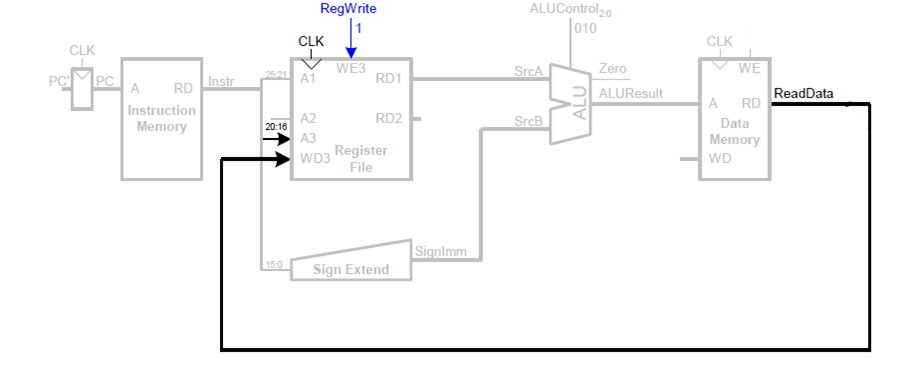
\includegraphics [width=17cm]{Prozessor4.png}
	\end{center}
	\caption{Memory und Write-Back}
\end{figure}

In dieser Abbildung wird der Pfad eines load-word (lw) Befehl gezeigt, bei dem ein Datum aus dem Arbeitsspeicher (Datenspeicher) geladen wird. Zuerst wurde die Adresse, die in einem Register gespeichert wurde, durch die ALU an den Adress-Eingang des Arbeitsspeichers gelegt. (Es kann bei dem Durchqueren der ALU noch ein immediate-Offset addiert werden.) Daraufhin wird das Datum, das aus dem Arbeitsspeicher kommt, in ein Register gespeichert.

\subsection{Program-Counter erhöhen}
\begin{figure}[H]
	\begin{center}
		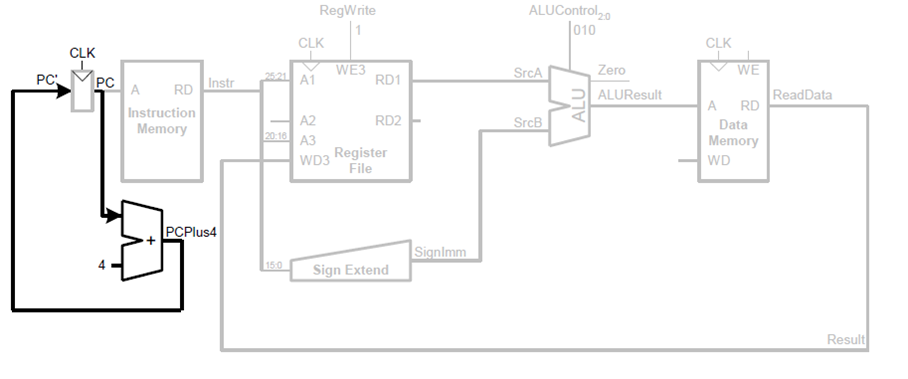
\includegraphics [width=17cm]{Prozessor5.png}
	\end{center}
	\caption{PC erhöhen}
\end{figure}

Während diese Berechnungen durchgeführt werden, wird der PC erhöht, damit bei der nächsten Ausführung nicht mehr der gleiche Befehl, sondern der darauffolgende ausgeführt wird. Dabei ist zu beachten, dass ein Befehl in 32 Bit kodiert ist und daher der PC um 4 Byte = 32 Bit erhöht werden muss. 

\subsection{Ohne Memory-Zugriff}
\begin{figure}[H]
	\begin{center}
		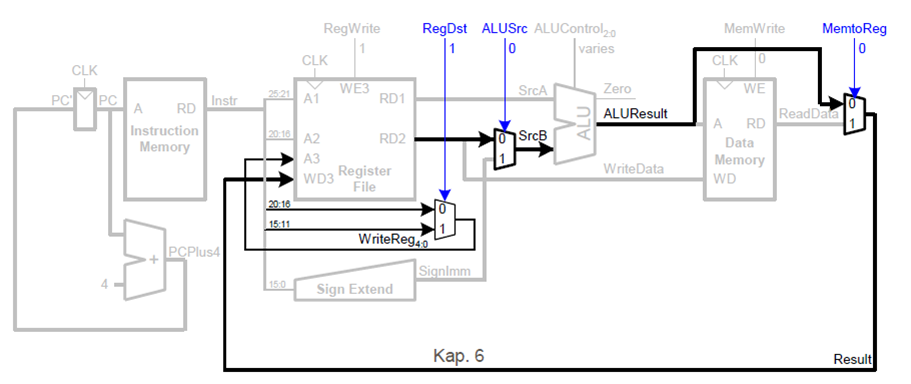
\includegraphics [width=17cm]{Prozessor6.png}
	\end{center}
	\caption{Laden aus zweitem Register}
\end{figure}

Bei dem Befehl für die Addition, den ich im MIPS-Kapitel vorgestellt habe, werden zwei Register geladen, addiert und in ein Register geschrieben. Dieser Pfad ist in dieser Abbildung eingezeichnet. Zu beachten ist, dass der Multiplexer, auf den der blaue "ALUSrc"-Pfeil zeigt, den zweiten Registerwert statt den immediate-Wert auswählt. In diesem Fall wird das Ergebnis von der Addition auch nicht als Adresse verwendet, sondern direkt in das Ziel-Register geschrieben.

\subsection{Branch}
\begin{figure}[H]
	\begin{center}
		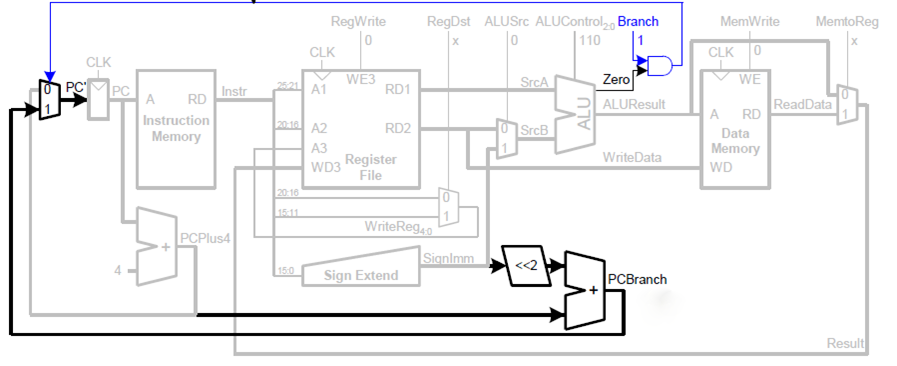
\includegraphics [width=17cm]{Prozessor7.png}
	\end{center}
	\caption{Branch-Pfad, mit dem der PC verändert wird}
\end{figure}

Bisher wurde der PC immer um eine Zeile erhöht, aber mit dem Branch Befehl muss es eine Möglichkeit geben, die den PC ändert. Dies wird über einen immediate-Wert umgesetzt. Dieser gibt ein Offset an, um das sich der PC ändern soll. z.B. "Springe 4 Befehle zurück" = -4 Also wird einfach ein Addierer verwendet, um diese Zahl auf den aktuellen PC zu addieren (ja, Addierer können auch subtrahieren, wenn man negative Zahlen eingibt, aber das werde ich hier nicht behandeln). Jetzt muss noch bestimmt werden, ob der Sprung überhaupt ausgeführt werden soll. Bei einem beq (branch-if-equal) Befehl, wie ich ihn oben vorgestellt habe, wird dies über Subtraktion gelöst. Die zwei Zahlen aus den Registern werden subtrahiert. Im Anschluss wird mit dem Zero-Ausgang der ALU getestet, ob das Ergebnis = 0 ist, was genau dann der Fall ist, wenn die beiden Zahlen gleich waren. Mit diesem Signal wird dann ausgewählt, ob der PC sich normal erhöhen	soll oder der Sprung-Wert als nächstes in den PC gespeichert werden soll.

\subsection{Kontrollpfad}
\begin{figure}[H]
	\begin{center}
		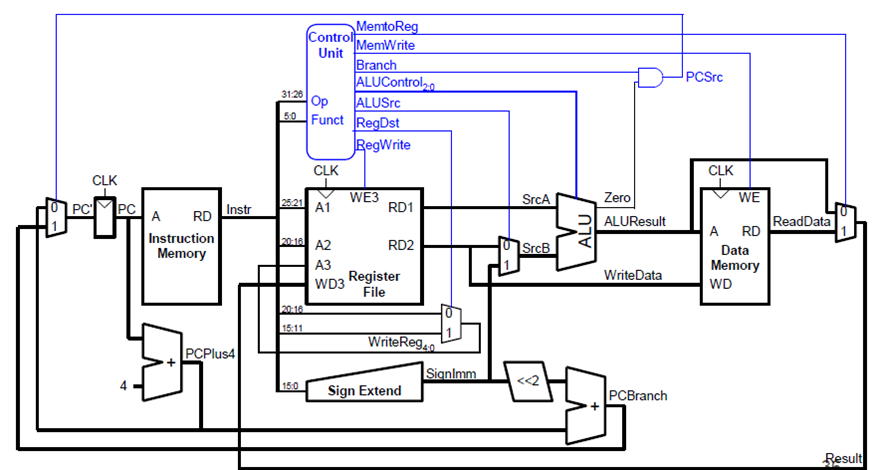
\includegraphics [width=17cm]{Prozessor8.png}
	\end{center}
	\caption{Kontrollpfad des Prozessors}
\end{figure}

Der Prozessor muss als letztes noch irgendwie gesteuert werden. Vermutlich sind in den letzten Abbildungen schon die blauen Pfeile aufgefallen, die "aus dem Nichts" kamen und die einzelnen Komponenten des Prozessors angesteuert haben. Einer dieser Pfeile hat z.B. gesteuert, ob der immediate-Wert oder der Wert aus dem zweiten Register zur Berechnung in der ALU verwendet werden soll. Diese blauen Signale werden in der Control-Unit aus einigen Bit des Befehls berechnet und steuern damit den kompletten Prozessor.

\section{Pipelining}
Um den Ablauf im Prozessor nochmal zusammenzufassen, kann man ihn in grobe 5 Phasen unterteilen:

\begin{table}[H]
	\begin{tabular}{ll}
		1. Instruction-Fetch:&Der Befehl wird mit dem PC geladen \\
		2. Register-Fetch:&Die Daten werden aus den Registern geladen \\
		3. Execute:&Die Rechenoperation wird ausgeführt \\
		4. Memory-Access:&Interaktion mit dem Arbeitsspeicher \\
		5. Write-Back:&Das Ergebnis wird in ein Register geschrieben \\
	\end{tabular}\\
\end{table}

Diese Phasen werden von den unterschiedlichen Bauteilen nacheinander abgearbeitet, wie das Bild unten darstellt.

\begin{figure}[H]
	\begin{center}
		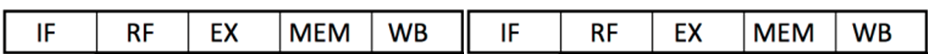
\includegraphics [width=11cm]{keinPipelining.png}
	\end{center}
	\caption{Ineffiziente Ausführung (Die Zeitachse verläuft nach rechts)}
\end{figure}

Während beispielsweise die Memory-Access Phase ist, hat die ALU nichts zu bearbeiten. Da fällt schnell auf, dass man dies verbessern kann, indem man bereits den zweiten Befehl anfängt abzuarbeiten, bevor der erste fertig ist. Dies sieht man grob in dem unteren Bild:

\begin{figure}[H]
	\begin{center}
		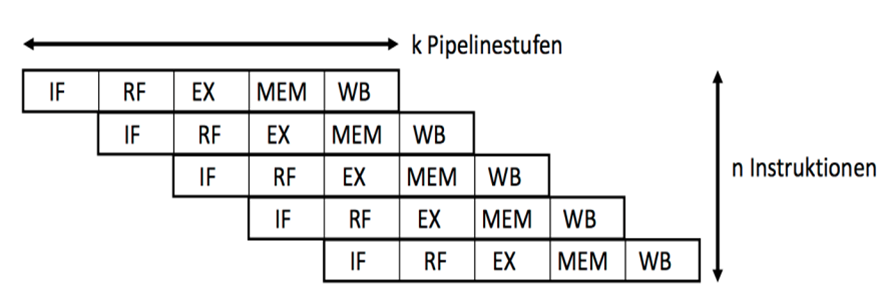
\includegraphics [width=15cm]{Pipelining.png}
	\end{center}
	\caption{Ausführung mit Pipelining (Die Zeitachse verläuft nach rechts)}
\end{figure}

Für dieses Pipelining muss die Architektur, die ich im letzten Kapitel vorgestellt habe, ein bisschen verändert werden. Wie in der nächsten Abbildung zu sehen, muss man mehrere große Register (die mit den blauen gestrichelten Linien) zwischen den Phasen einfügen, damit die Ergebnisse von der einen zur nächsten Phase gespeichert werden können.

\begin{figure}[H]
	\begin{center}
		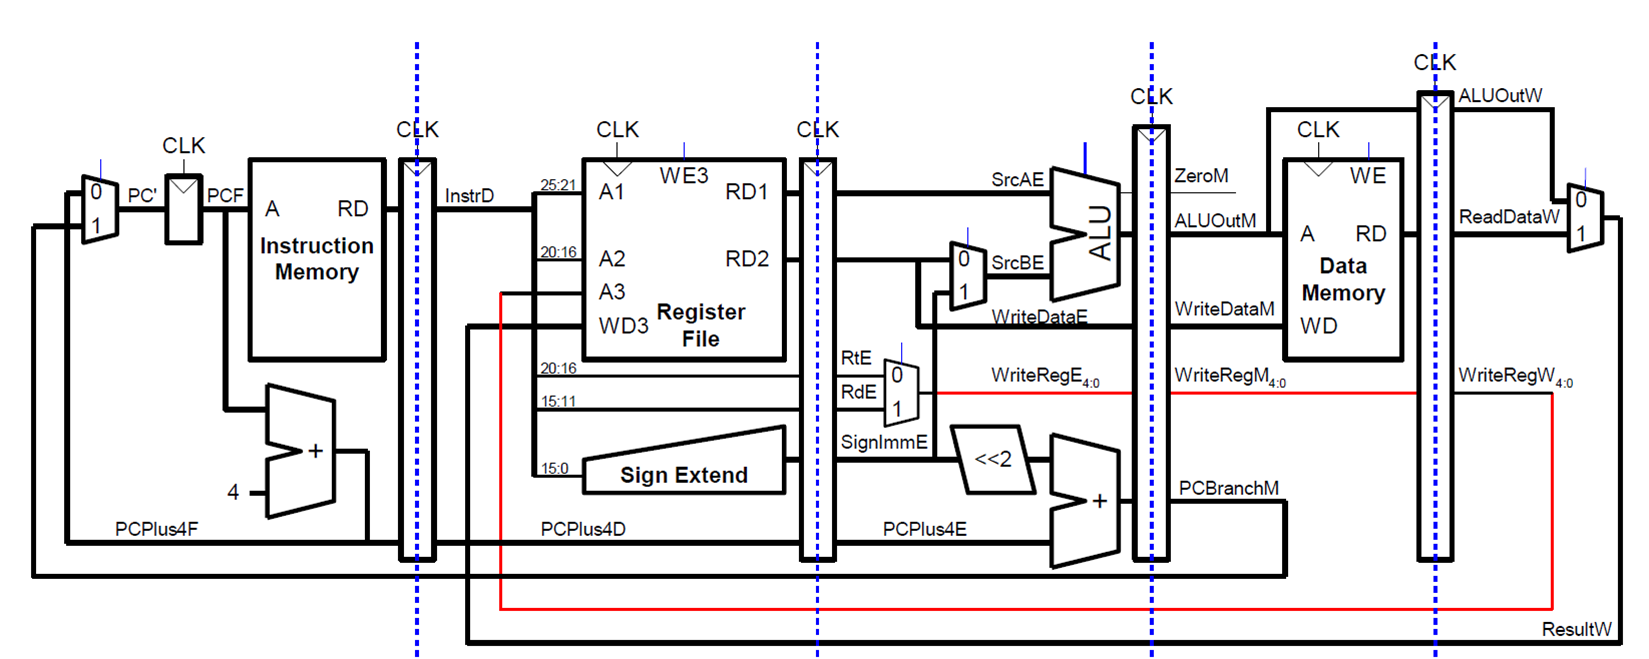
\includegraphics [width=17cm]{Prozessor9.png}
	\end{center}
	\caption{Ausführung mit Pipelining (Die Zeitachse verläuft nach rechts)}
\end{figure}

\subsection{Read-after-write Hazard}
Beim Pipelining muss man jedoch noch so genannte Hazards beachten, die Probleme verursachen können, wenn man sie nicht beachtet. Beispielsweise kann es passieren, dass ein Befehl die Ergebnisse des vorherigen Befehls benötigen. Dieser Befehl wird beim Pipelining einfach ausgeführt, bevor der vorherige Befehl fertig ist und lädt einen falschen Wert aus dem Register, da der letzte Befehl sein Ergebnis noch nicht in das entsprechende Register gespeichert hat.

\subsection{Branch oder nicht?}
Ein anderes Problem könnte das Branching sein. Was passiert, wenn nach dem Branch-Befehl schon die nächsten zwei Befehle halb ausgeführt werden, bevor festgestellt wird, dass eigentlich an eine ganz andere Programmstelle gesprungen werden soll und die Befehle von dort ausgeführt werden sollen.

\subsection{Lösungsmöglichkeiten von Hazards}
Es können zwischen zwei Befehlen, die von Hazards betroffen sind, so genannte NOPs (no-Operations) einfügen, die einfach nichts machen. Dadurch muss der zweite Befehl noch warten, bis das Ergebnis des ersten Befehls da ist. Eine andere Strategie, die angewendet wird, ist bestimmte Informationen schon vorzuschleusen. Das heißt, dass z.B. die Information, ob ein Branch durchgeführt werden soll bereits nach der Execute-Phase verfügbar und muss nicht noch warten, bis die Memory und die Write-Back Phasen abgeschlossen sind. Die letzte und komplizierteste Strategie, die ich hier vorstellen werde ist die branch-prediction. Hierbei versucht der Prozessor intelligent zu raten, ob ein Branch durchgeführt werden wird oder nicht. Dies geschieht auf Basis von vorherigen Ausführungen des gleichen Befehls. Wenn eine Schleife beispielsweise 1000 Mal durchgeführt wird. wird der Prozessor im optimalen Fall nach dem 3. Sprung an den Schleifenanfang merken, dass er auf "Sprung" tippen kann und lädt die Befehle vom Schleifenanfang schon vor, statt auf das Ergebnis des Branch-Befehls zu warten. Jedoch kann es dann vorkommen, dass sich der Prozessor vertippt und den falschen Branch vorlädt. In diesem Fall muss die komplette Pipeline geleert werden, damit der Code von dem anderen Branch eingefügt werden kann. Dies passiert allerdings sehr selten, da die Sprünge in einem Programm sehr vorhersehbar sind.

\section{Literatur}
Mir hat die Vorlesung Systemarchitektur von Professor Jan Reineke an der Universität des Saarlandes am meisten geholfen, diesen Stoff zu verstehen. Aus den Folien der Vorlesung habe ich auch die meisten Abbildungen, die ich hier verwendet habe. Niki und Florian haben folgende Literatur empfohlen:
\begin{enumerate}
	\item Computer Organization and Design, The Hardware/Software Interface
	\item Computer Architecture: A Quantitative Approach
	\item Inside the Machine: An Illustrated Introduction to Microprocessors and Computer Architecture
\end{enumerate}

\end{document}